\documentclass[11pt]{article}
\usepackage[margin=1in]{geometry}
\usepackage{amsmath,amssymb}
\usepackage{booktabs}
\usepackage{graphicx}
\usepackage{xcolor}
\usepackage[hidelinks]{hyperref}
\usepackage{caption}
\usepackage{microtype}
\usepackage{enumitem}
\usepackage{fancyhdr}
\usepackage{titlesec}

\definecolor{acc}{HTML}{1F6F8B}
\definecolor{bad}{HTML}{C0392B}
\newcommand{\code}[1]{\texttt{\small #1}}
\newcommand{\fail}[1]{\textcolor{bad}{\textbf{#1}}}
\newcommand{\pass}[1]{\textcolor{acc}{\textbf{#1}}}

\pagestyle{fancy}\fancyhf{}
\fancyhead[L]{\small Controls on a stale-state internal-representation claim}
\fancyfoot[C]{\small\thepage}
\renewcommand{\headrulewidth}{0.4pt}

\title{\bfseries Controls on an Internal-Representation Claim\\[2pt]
\large Stale-State Tracking Failures in Qwen: Why a 137/137 Result Does Not Hold,\\and What Survives in Its Place}
\author{Tarun Nagaraju\thanks{Analysis and controls performed with Claude Opus 5. All results are
reproducible from committed CSVs; no GPU required.}}
\date{September 2026}

\begin{document}
\maketitle

\begin{abstract}
\noindent
A mechanistic-interpretability probe of stale-state tracking in Qwen reported that
\emph{in 137 of 137 stale-output failures, the correct state outranks the stale state in at
least one internal layer}, and concluded that the correct state is encoded internally but
goes unused at the output. Because that statistic is a maximum over 29 layers, it requires
controls. We run four. The claim does not survive any of them. The reverse statistic ---
the stale state outranking the correct state --- also holds in 137/137 failures; the same
test fires in 488/488 successes, giving it zero discriminative power; and a permutation
null shows the statistic is \emph{invariant} under swapping the correct/stale labels, so it
is untestable rather than merely weak. Its graded form is significant in the direction
opposite the claim. We further show that two previously reported figures, a mean best rank
of $47{,}343$ and of $2.3$, are the same lens on the same 137 examples and differ only in
the layer set swept; the favourable number arises entirely from including near-output
layers, where the correct state is the runner-up to a stale state already at rank~1.
Separately, we identify a severe condition confound: every failure is a
complexity-3, agent-entity, middle-distractor item, while $70\%$ of successes contain no
distractors at all. After matching on condition and correcting for layer selection, two
signals survive: attention mass differential at layer~22 (AUC $0.973$, held-out $0.970$)
and J-lens margin at layer~5 (AUC $0.888$, held-out $0.882$). Logit-lens margin does not
survive: it passes a permutation null but its best layer is reproducible in only $32\%$ of
splits. All surviving results are correlational.
\end{abstract}

\section{Introduction}

The claim under test is:

\begin{quote}
\itshape In 137/137 stale-output failures, the correct room outranks the stale room in at
least one internal layer.
\end{quote}

and the interpretation attached to it: that the updated state is present in the model's
internal representations while the model emits the stale one --- an \emph{expression} or
readout failure rather than a representational one.

The statistic has a specific structural weakness. It is an \emph{existence} test evaluated
as a maximum over layers: an example counts as supporting the claim if there is
\emph{any} layer at which the correct state's rank is lower than the stale state's. With 29
layers of noisy rank measurements, two exchangeable series will satisfy such a test almost
surely. A result of $137/137$ is therefore not by itself evidence of anything; it is the
expected outcome under a wide range of nulls, including nulls in which the correct state is
never meaningfully represented.

This paper reports four controls (Section~\ref{sec:round1}), a confound that invalidates the
original failure-vs-success comparison (Section~\ref{sec:confound}), and a matched,
selection-corrected re-analysis (Section~\ref{sec:round2}). Section~\ref{sec:survive} states
what survives. Section~\ref{sec:limits} states what these data cannot establish.

\paragraph{Contributions.}
\begin{enumerate}[leftmargin=*,itemsep=1pt]
\item Four controls showing the headline statistic is vacuous, including a permutation null
      under which it is provably invariant.
\item A reconciliation of two conflicting published figures ($47{,}343$ vs $2.3$) as an
      artifact of layer-set selection, not of lens choice.
\item Identification and correction of a complete condition confound between the failure and
      success populations.
\item A matched, selection-corrected re-analysis isolating two surviving signals and
      falsifying a third.
\end{enumerate}

\section{Data}
\label{sec:data}

Three CSV exports, all derived from a single 5{,}000-record dataset. Their relationship was
not documented and had to be reconstructed.

\begin{table}[h]
\centering\small
\begin{tabular}{lrrl}
\toprule
Run & Examples & Layers & Outcomes \\
\midrule
\code{colab\_run\_qwen\_5k\_L5-8-13}         & 5{,}000 & 3 (5, 8, 13) & 4{,}853 correct / 137 stale / 10 other \\
\code{colab\_run\_qwen\_fullsweep\_500}      & 500     & 29 (0--28)   & 488 correct / 12 stale \\
\code{colab\_run\_qwen\_failures\_fullsweep} & 137     & 29 (0--28)   & 137 stale \\
\bottomrule
\end{tabular}
\caption{The three runs. The 500-record run is a subset of the 5k dataset; the 137-failure
run is the complete failure population of the same dataset.}
\end{table}

\paragraph{Layer count.} The sweeps contain \textbf{29} layers, indexed $0$--$28$, not 28.
The maximum in the headline statistic is therefore over 29 draws.

\paragraph{Provenance reconstruction.} The 137-failure export renumbered
\code{dataset\_index} to $0\ldots136$, making it appear disjoint from the 5k run under an
index join. Matching per-example rank signatures at the three shared layers recovers the
true indices for $137/137$ examples, all signatures unique. The 137-failure file is exactly
the stale subset of the 5k run.

\paragraph{Poolability.} Twelve examples appear in both 29-layer files. All rank columns
agree \emph{exactly} on these, so the two files are measurement-compatible and pool into a
single contrast of \textbf{137 failures against 488 successes at full depth}. An earlier
analysis used only the 12 failures inside the 500-record run; this was an avoidable loss of
power, as 137 were available throughout.

\paragraph{Measures.} Each row carries two lens families and an attention block.
\emph{Logit lens} decodes a residual stream state as
$\mathrm{lm\_head}(\mathrm{final\_norm}(h_i))$. \emph{J-lens} decodes it through a
first-order expansion of the model's own remaining computation,
$\mathrm{jlens}_i = f_i(b) + J\,(h_i - b)$ with $b=0$, where $f_i$ runs decoder layers
$i \ldots 28$, the final norm, and the unembedding, using the real frozen KV cache. Nine
\code{attn\_*} columns record attention mass at the readout position. Ranks are
0-indexed positions in the vocabulary distribution; \emph{lower is better}, and
``outranks'' means strictly smaller rank. The observed maximum rank implies a vocabulary
lower bound of $V = 152{,}065$.

\section{Round 1: Four Controls}
\label{sec:round1}

\subsection{Control 1 --- Symmetry}

If the existence test also fires in the reverse direction, it carries no directional
information.

\begin{table}[h]
\centering\small
\begin{tabular}{lrrr}
\toprule
Group ($n$) & correct wins $\geq 1$ layer & stale wins $\geq 1$ layer & both \\
\midrule
137 stale failures (logit lens) & $137/137 = 100.0\%$ & \fail{$137/137 = 100.0\%$} & $100.0\%$ \\
137 stale failures (J-lens)     & $137/137 = 100.0\%$ & \fail{$137/137 = 100.0\%$} & $100.0\%$ \\
\bottomrule
\end{tabular}
\caption{Symmetry control. The test fires in both directions in every single example.}
\end{table}

In the median failure the correct state wins at 9 of 29 layers and the stale state wins at
20. The existence test is satisfied by any two rank series that cross even once.

\subsection{Control 2 --- Discrimination}

If successes also saturate, the statistic cannot separate the outcome it purports to explain.

\begin{table}[h]
\centering\small
\begin{tabular}{lrrr}
\toprule
Group & $n$ & correct wins $\geq 1$ layer & mean layers won \\
\midrule
\code{fullsweep\_500} successes & 488 & \fail{$100.0\%$} & 18.0 \\
137-failure run                 & 137 & $100.0\%$        & 10.9 \\
\midrule
\multicolumn{2}{l}{\itshape Delta (failures $-$ successes)} & \fail{$+0.0$ pp} & \\
\bottomrule
\end{tabular}
\caption{Discrimination control (logit lens; J-lens identical at $100.0\%$ both arms).}
\end{table}

The statistic has exactly zero discriminative power. Note that the \emph{graded} form ---
the number of winning layers --- does differ between groups (18.0 vs 10.9). That is a
different statistic than the one claimed, and Section~\ref{sec:confound} shows this
particular contrast is confounded.

\subsection{Control 3 --- Magnitude, and a reconciliation}
\label{sec:magnitude}

Two figures had been reported for the mean best rank of the correct state: $47{,}343$ and
$2.3$. These are \emph{not} different lenses and \emph{not} different examples. They are the
same lens (logit lens) on the same 137 examples, differing only in the set of layers over
which the minimum is taken.

\begin{table}[h]
\centering\small
\begin{tabular}{lrr}
\toprule
Minimum taken over & mean best rank & median \\
\midrule
layers $\{5, 8, 13\}$ (the 3-layer run) & $47{,}343.5$ & $44{,}626$ \\
layers $\{0 \ldots 28\}$ (full sweep)   & $2.3$        & $2$ \\
\bottomrule
\end{tabular}
\caption{The entire difference is layer-set selection. Restricting the full sweep to
$\{5,8,13\}$ reproduces $47{,}343.5$ to the decimal.}
\end{table}

The improvement comes entirely from admitting near-output layers, and inspecting where the
minimum occurs shows why this cannot support the claim:

\begin{itemize}[leftmargin=*,itemsep=1pt]
\item The best rank occurs at layer $\geq 26$ in \textbf{100\%} of failures (layer 28: 115
      examples; layer 27: 21; layer 26: 1).
\item At that layer the correct state outranks the stale state in only \textbf{13.1\%} of
      failures. The median stale rank there is \textbf{1} and the median correct rank is
      \textbf{2}: the correct state is the \emph{runner-up at the output}, which is what a
      stale failure is by definition.
\item Where the correct state genuinely wins by the largest margin (median layer 9), both
      tokens are buried: median correct rank $24{,}183$ against stale rank $103{,}440$, out
      of $V \approx 152{,}065$.
\end{itemize}

These two regimes are disjoint. The headline result is assembled by taking the existence
test from the deep-tail regime and the impressive rank number from the output regime. For
calibration, the expected minimum of 29 i.i.d.\ uniform draws over the vocabulary is
$(V-1)/30 \approx 5{,}069$.

\subsection{Control 4 --- Depth profile}

\begin{figure}[h]
\centering
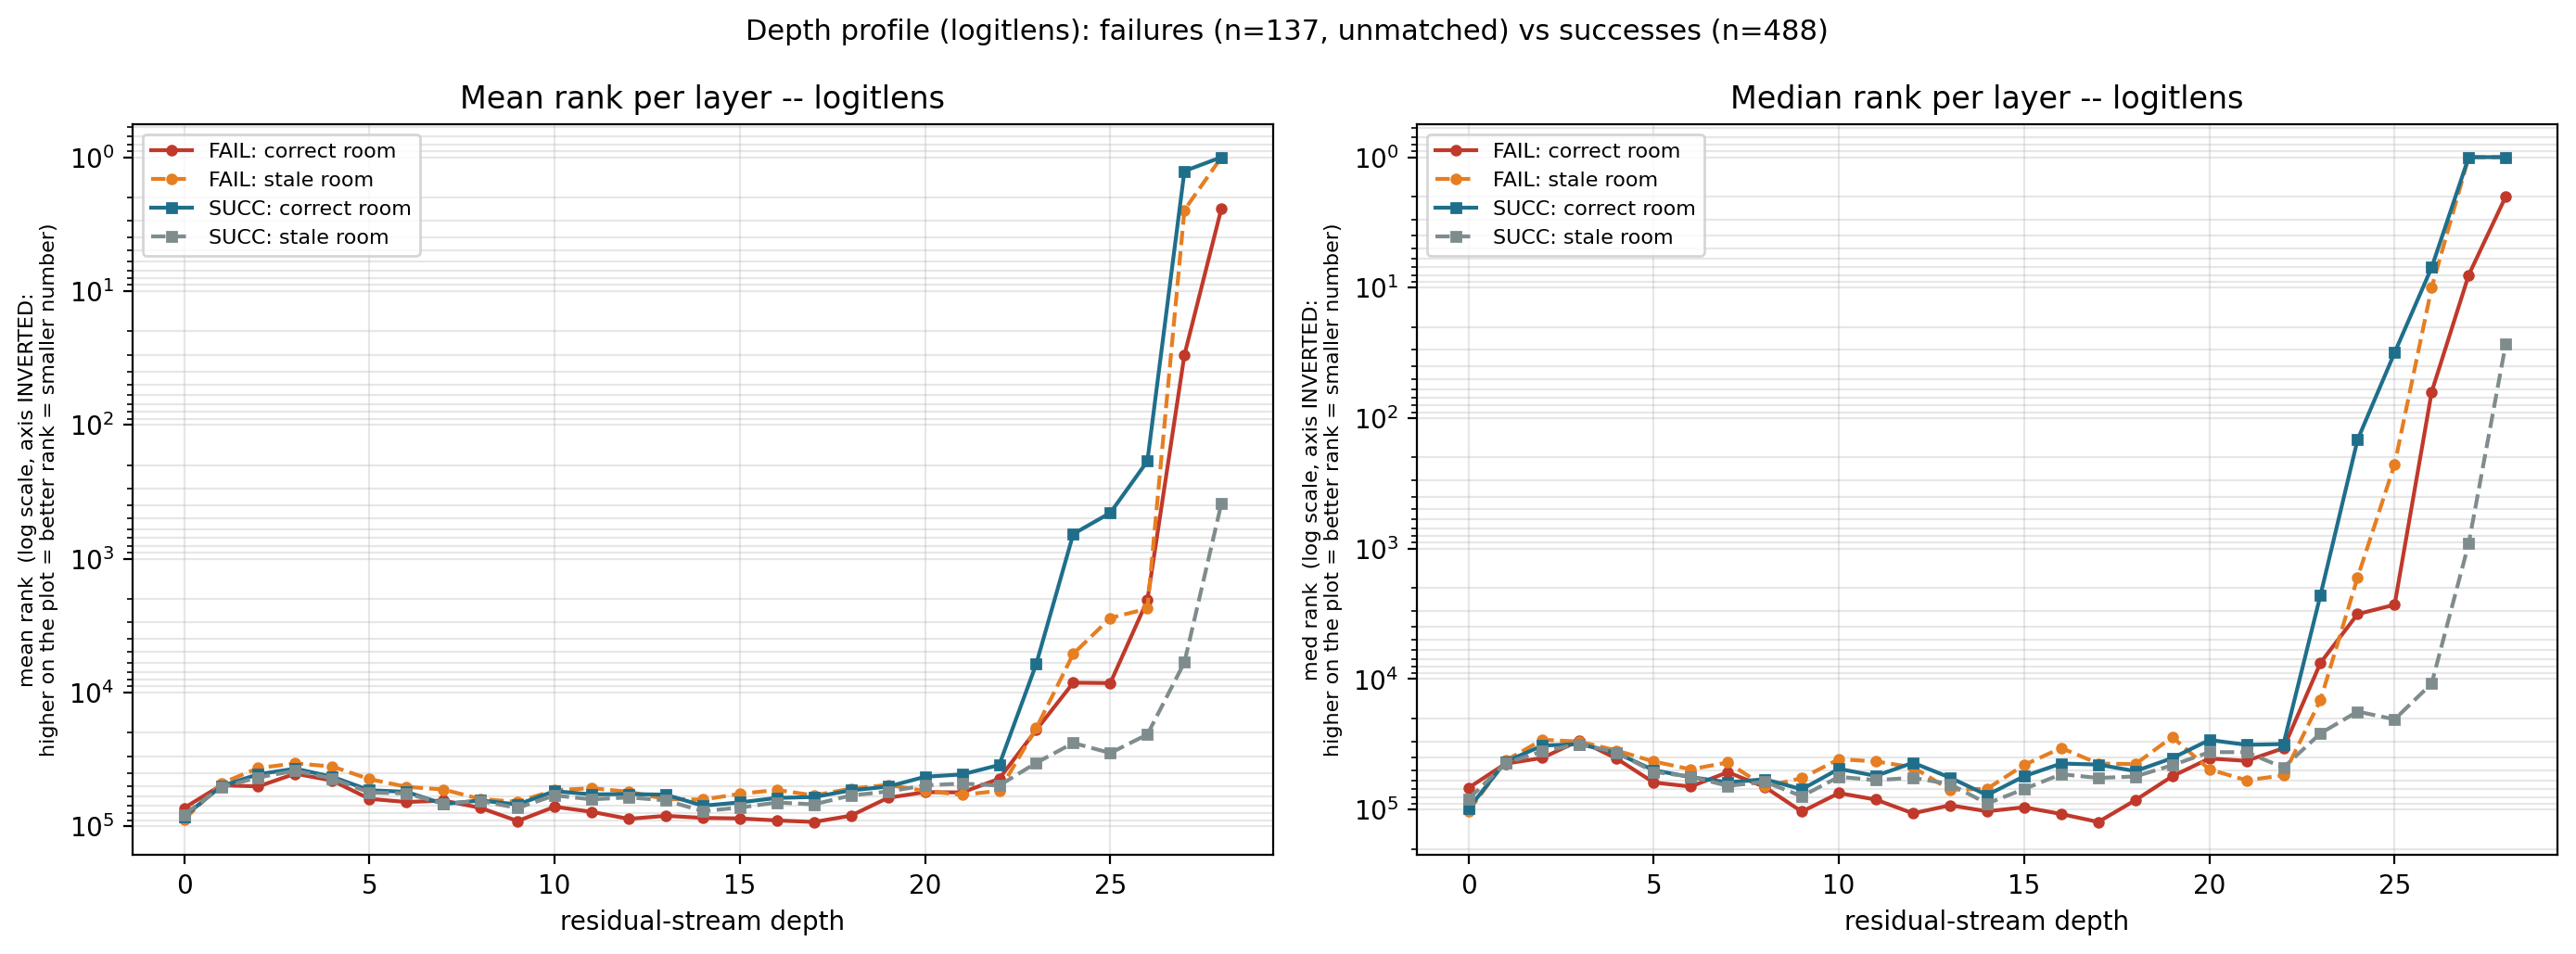
\includegraphics[width=\textwidth]{../reports/depth_profile_logitlens.png}
\caption{Mean and median rank per layer, failures versus successes (logit lens; ranks
inverted so better is higher). All four curves overlap around rank $10^5$ through layer
$\sim21$ and separate only in the final five to six layers. Unmatched groups; see
Section~\ref{sec:confound}.}
\end{figure}

Averaged over layers 0--23, the mean gap (stale rank minus correct rank; positive favours
the correct state) is $\mathbf{-14{,}575}$ in failures and $+5{,}067$ in successes. In
failures the gap remains negative even over the last five layers ($-1{,}751$). Through most
of the stack the stale state is \emph{better} ranked than the correct state --- the opposite
of the claim's spirit.

\begin{figure}[h]
\centering
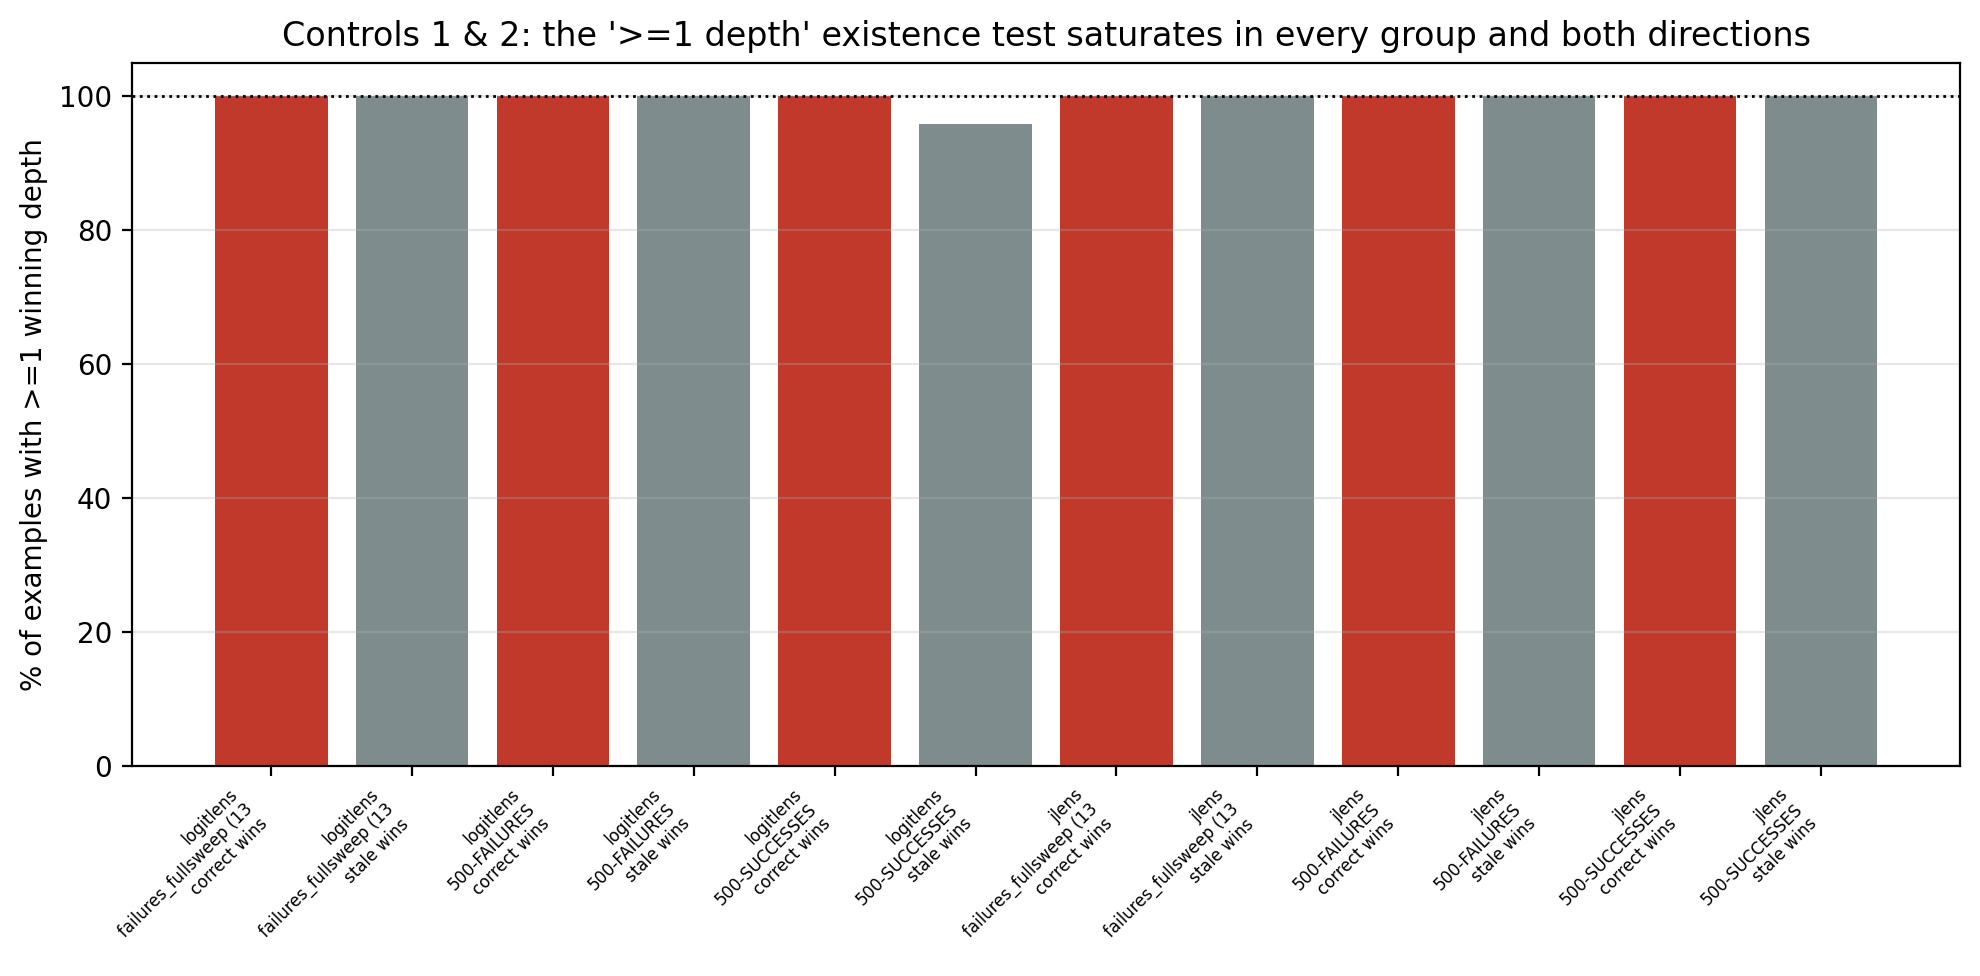
\includegraphics[width=0.86\textwidth]{../reports/control_saturation.png}
\caption{Controls 1 and 2 together: the existence test saturates at or near $100\%$ in every
group and in both directions.}
\end{figure}

\section{A Condition Confound}
\label{sec:confound}

Every failure-vs-success comparison above compares populations that differ systematically in
task condition.

\begin{table}[h]
\centering\small
\begin{tabular}{lrr}
\toprule
Condition & Failures & Successes \\
\midrule
\code{complexity\_level} $=3$        & \fail{$100\%$} & $29.3\%$ \\
\code{n\_distractors} $\geq 3$       & \fail{$100\%$} & $29.3\%$ \\
\code{distractor\_position} = middle & \fail{$100\%$} & $29.3\%$ \\
\code{entity\_type} = agent          & \fail{$100\%$} & $52.5\%$ \\
\bottomrule
\end{tabular}
\caption{Every failure is a hard, agent-entity, middle-distractor item. Roughly $70\%$ of
successes contain no distractors at all.}
\end{table}

Any measure correlated with task difficulty will separate these groups for reasons unrelated
to the outcome. We therefore define a \textbf{matched stratum}: \code{complexity\_level}$=3$,
\code{entity\_type}$=$agent, \code{distractor\_position}$=$middle,
\code{n\_distractors}$\in\{3,4\}$. These constraints are collinear in this dataset: the
first two alone select the same records. The stratum retains $72$ of $488$ successes in the
29-layer run and $682$ of $4{,}853$ in the 5k run; all 137 failures already lie inside it.
The 72 coincide with an earlier stale-mention-count matching, reached independently.

Two clarifications on scope. Controls 1 and 3 are \emph{within-failure} analyses and are
untouched by this confound. Control 2's headline conclusion also stands regardless: a
statistic sitting at $100\%$ in both arms cannot be rescued by rebalancing. What the
confound invalidates is every \emph{magnitude} --- the graded layer counts, the depth-profile
separations, and all AUCs computed on unmatched groups.

\section{Round 2: Matched, Selection-Corrected Controls}
\label{sec:round2}

\subsection{Raw versus matched}

\begin{figure}[h]
\centering
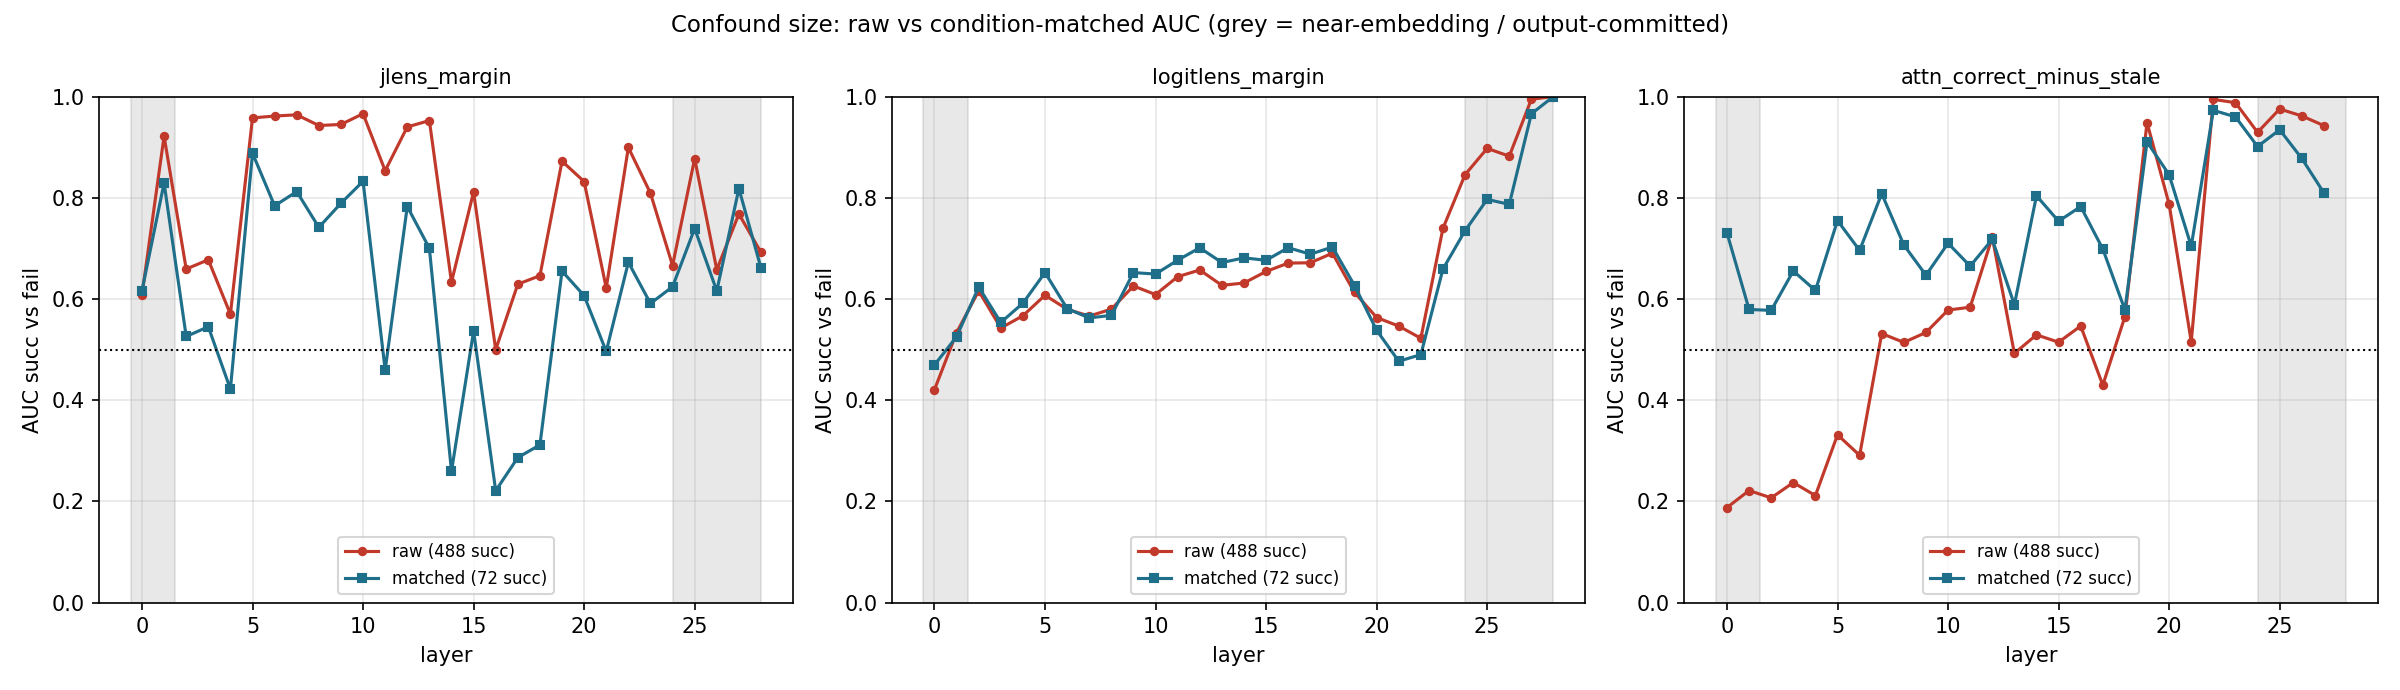
\includegraphics[width=\textwidth]{../reports/auc_raw_vs_matched.png}
\caption{Per-layer AUC separating success from failure, raw (488 successes) versus matched
(72). Shaded bands mark near-embedding layers 0--1 and output-committed layers 24--28, where
an AUC is circular: at layer 28 the lens \emph{is} the model's decision, and indeed measures
exactly $1.000$ there.}
\end{figure}

\begin{table}[h]
\centering\small
\begin{tabular}{lrrrr}
\toprule
Measure & Layer & Raw AUC & Matched AUC & Shrinkage \\
\midrule
\code{jlens\_margin}             & 5  & 0.958 & 0.888 & $-0.070$ \\
\code{attn\_correct\_minus\_stale} & 19 & 0.949 & 0.910 & $-0.039$ \\
\code{attn\_correct\_minus\_stale} & 22 & 0.994 & 0.973 & $-0.021$ \\
\bottomrule
\end{tabular}
\caption{Confound size at the layers of interest. Elsewhere in the mid-stack the shrinkage
is far larger: J-lens at layer 13 falls from $0.952$ to $0.700$.}
\end{table}

The 5k run provides a larger matched replication at its three layers ($682$ successes versus
$137$ failures): J-lens margin gives $0.883$, $0.743$, $0.681$ at layers 5, 8, 13, against
logit-lens $0.617$, $0.573$, $0.616$.

\subsection{Permutation nulls}

Two distinct exchangeability assumptions are at stake, and conflating them is how a
max-over-layers statistic acquires spurious significance.

\paragraph{Null A --- correct/stale label swap.} For each example, swap the correct and
stale rank series across \emph{all} 29 layers at once. This encodes ``which state is the
correct one carries no information.'' The whole-series swap is required: swapping
independently per layer would destroy within-example cross-layer correlation and yield a
falsely narrow null for a maximum statistic. This is the null for the original claim.

\begin{table}[h]
\centering\small
\begin{tabular}{llrrr}
\toprule
Statistic & Lens & Observed & Null & $p$ \\
\midrule
Fraction winning $\geq 1$ of 29 layers & logit & $1.0000$ & point mass at $1.0000$ & \fail{$1.00$} \\
Fraction winning $\geq 1$ of 29 layers & J-lens & $1.0000$ & point mass at $1.0000$ & \fail{$1.00$} \\
Mean layers won (graded)               & logit & $10.93$ & $14.48$\ \ $[13.12, 15.82]$ & \fail{$<10^{-4}$} \\
Mean layers won (graded)               & J-lens & $8.41$ & $14.34$\ \ $[13.15, 15.54]$ & \fail{$<10^{-4}$} \\
\bottomrule
\end{tabular}
\caption{Null A, 5{,}000 permutations. The existence statistic has a \emph{degenerate} null.}
\end{table}

Two findings, both fatal to the claim. First, the existence statistic's null is a
\textbf{point mass at $1.000$}: because both directions already hold in all 137 examples,
relabelling cannot change the value. The statistic is \emph{invariant} under the null and
therefore \textbf{untestable}, not merely non-significant. Second, the graded form is highly
significant \textbf{in the direction opposite the claim}: the correct state wins
\emph{fewer} layers ($10.93$) than label-exchange chance predicts ($14.48$).

\paragraph{Null B --- outcome label shuffle.} Shuffle failure/success labels across
examples and, within each permutation, take the maximum $|\mathrm{AUC}-0.5|$ over the
internal band (layers 2--23). Taking the maximum inside the permutation is what corrects for
having chosen the best layer.

\begin{table}[h]
\centering\small
\begin{tabular}{lrrrl}
\toprule
Measure & Best layer & $|\mathrm{AUC}-0.5|$ & Null 95th pct & $p$ \\
\midrule
\code{jlens\_margin}              & 5  & $0.388$ & $0.125$ & \pass{$<10^{-4}$} \\
\code{logitlens\_margin}          & 18 & $0.203$ & $0.117$ & \pass{$<10^{-4}$} \\
\code{attn\_correct\_minus\_stale} & 22 & $0.473$ & $0.123$ & \pass{$<10^{-4}$} \\
\bottomrule
\end{tabular}
\caption{Null B on matched groups (72 successes, 137 failures), 5{,}000 permutations.}
\end{table}

\begin{figure}[h]
\centering
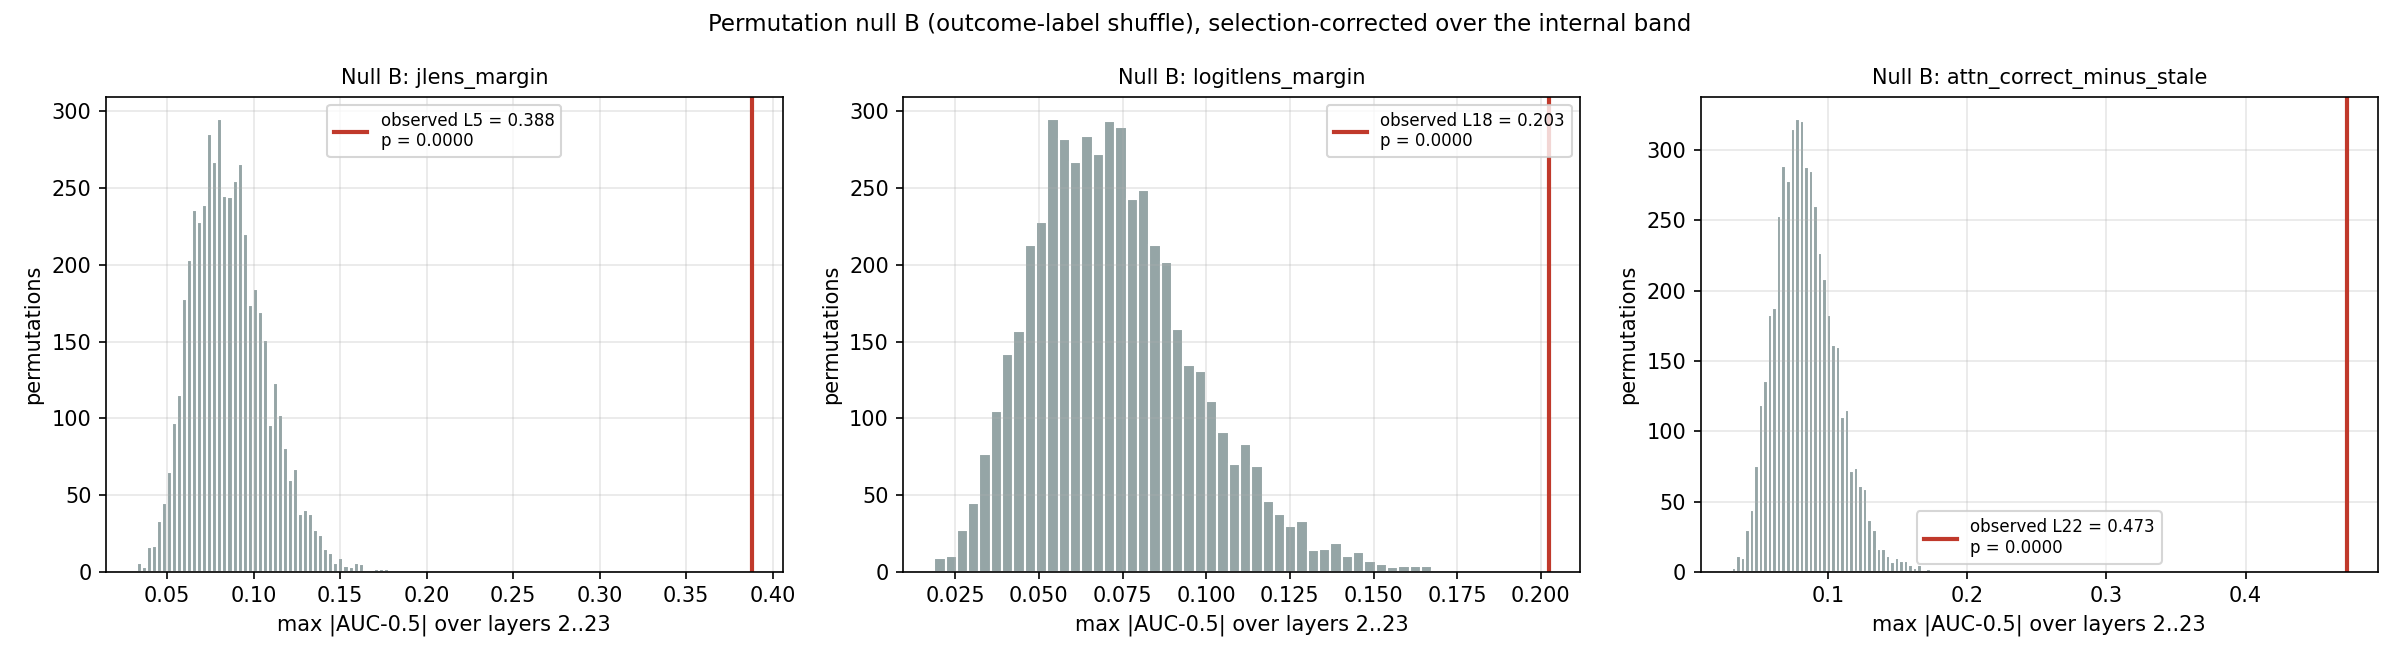
\includegraphics[width=\textwidth]{../reports/perm_null_B.png}
\caption{Null B distributions with observed values marked. All three measures clear the
selection-corrected null; stability is decided by the split-half test below.}
\end{figure}

\subsection{Split-half layer selection}

Passing a permutation null does not establish that a \emph{particular} layer carries the
effect. We select the best internal layer on one half of the matched data and evaluate it on
the held-out half, over 500 random splits, recording which layer gets selected each time.

\begin{table}[h]
\centering\small
\begin{tabular}{lrrrl}
\toprule
Measure & Modal layer & Held-out AUC (95\%) & Layer stability & Verdict \\
\midrule
\code{attn\_correct\_minus\_stale} & 22 & $0.970$\ \ $[0.939, 0.991]$ & $90\%$ & \pass{stable} \\
\code{jlens\_margin}              & 5  & $0.882$\ \ $[0.777, 0.935]$ & $96\%$ & \pass{stable} \\
\code{logitlens\_margin}          & 18 & $0.669$\ \ $[0.576, 0.747]$ & \fail{$32\%$} & \fail{unstable} \\
\bottomrule
\end{tabular}
\caption{Split-half, 500 splits. Halves contain $\sim$36 successes and $\sim$68 failures.}
\end{table}

\begin{figure}[h]
\centering
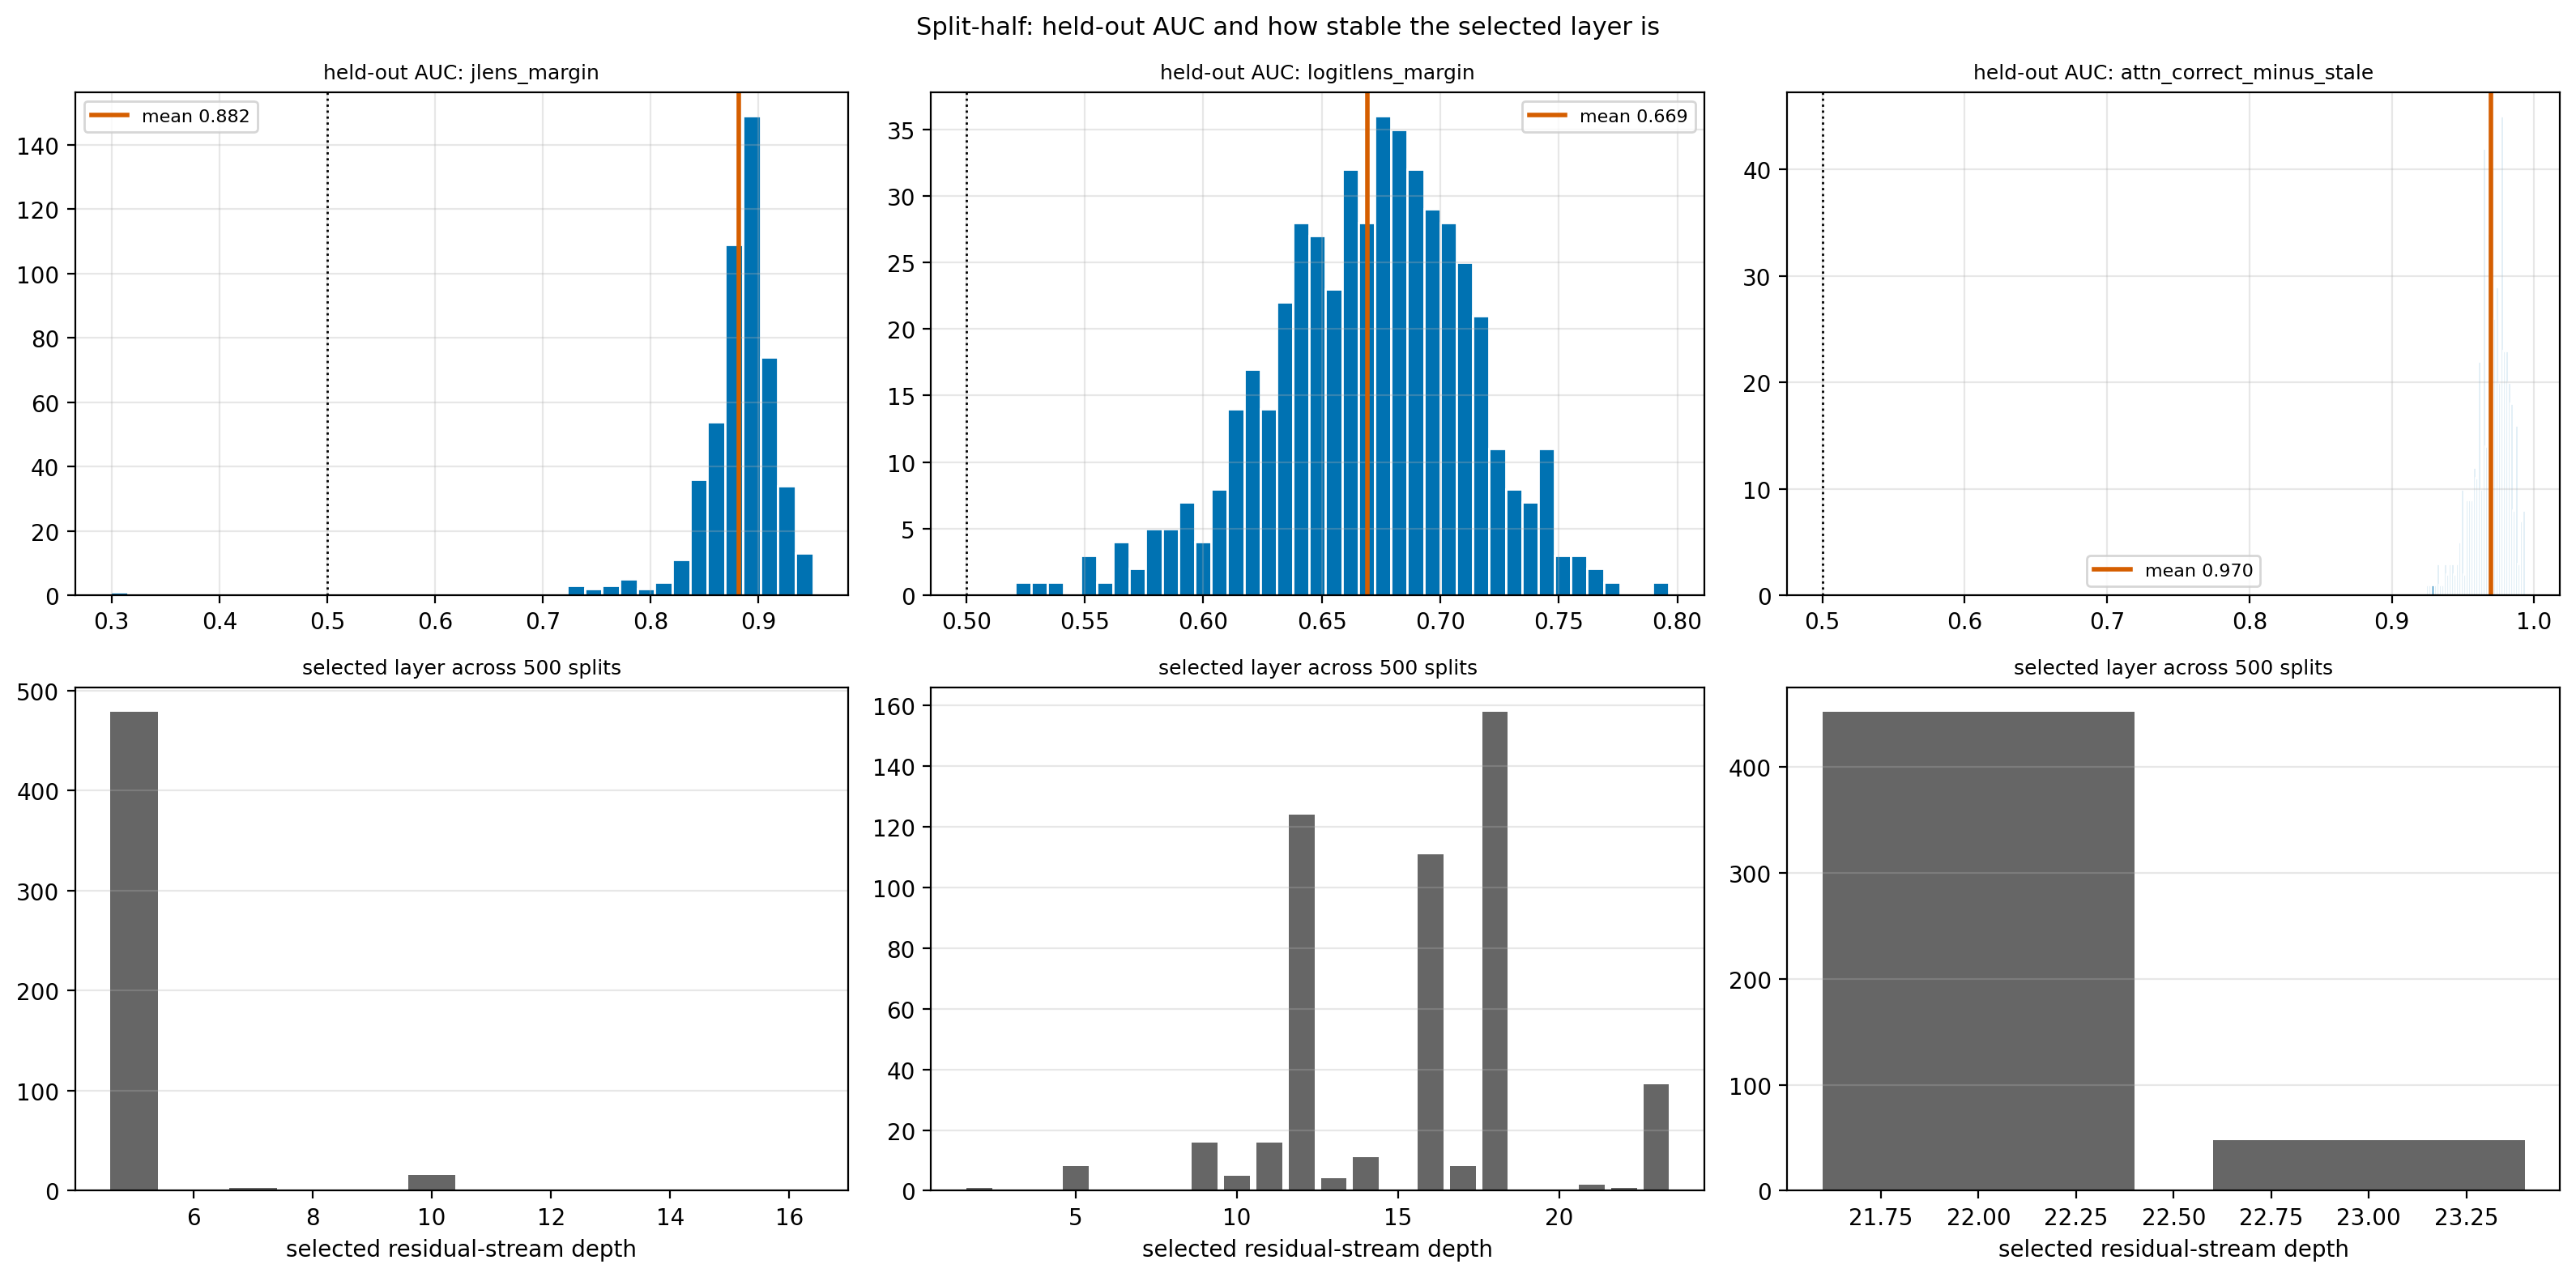
\includegraphics[width=\textwidth]{../reports/split_half.png}
\caption{Held-out AUC distributions (top) and selected-layer distributions (bottom). J-lens
and attention concentrate on a single layer; logit lens spreads across layers 12, 16, 18 and
23 with no reproducible locus.}
\end{figure}

Logit-lens margin therefore \textbf{fails}. It reflects a real but diffuse effect with no
reproducible best layer, and any claim naming a specific logit-lens layer is not supported.

\subsection{Attention sweep}

All nine \code{attn\_*} columns were previously unanalysed. We sweep them across all layers
on the matched groups.

\paragraph{Missing-data policy.} Layer 28 carries \emph{no} attention data in either file:
all nine columns are $100\%$ missing there, accounting for all $5{,}733$ attention NaNs.
Outside layer 28 nothing is missing. The sweep therefore covers layers 0--27 and reports
layer 28 as ``no data'' rather than filling, zeroing, or silently dropping it. Additionally,
within the matched stratum \code{attn\_stale\_mass} equals \code{attn\_stale\_anchor\_mass}
and \code{attn\_correct\_mass} equals \code{attn\_correct\_update\_mass}, because matched
records carry a single stale mention, so first-mention mass is total mass. The sweep thus
covers seven distinct measures, not nine.

\begin{table}[h]
\centering\small
\begin{tabular}{lrrr}
\toprule
Column & Layer & AUC & $|\mathrm{AUC}-0.5|$ \\
\midrule
\code{attn\_correct\_minus\_stale} & 22 & $0.973$ & $0.473$ \\
\code{attn\_stale\_mass}           & 22 & $0.030$ & $0.470$ \\
\code{attn\_correct\_minus\_stale} & 23 & $0.960$ & $0.460$ \\
\code{attn\_max\_head\_correct}    & 23 & $0.959$ & $0.459$ \\
\code{attn\_max\_head\_stale}      & 23 & $0.047$ & $0.453$ \\
\bottomrule
\end{tabular}
\caption{Top of the matched sweep. AUC below $0.5$ means the quantity is \emph{higher} in
failures, the expected direction for stale-directed attention.}
\end{table}

\begin{figure}[h]
\centering
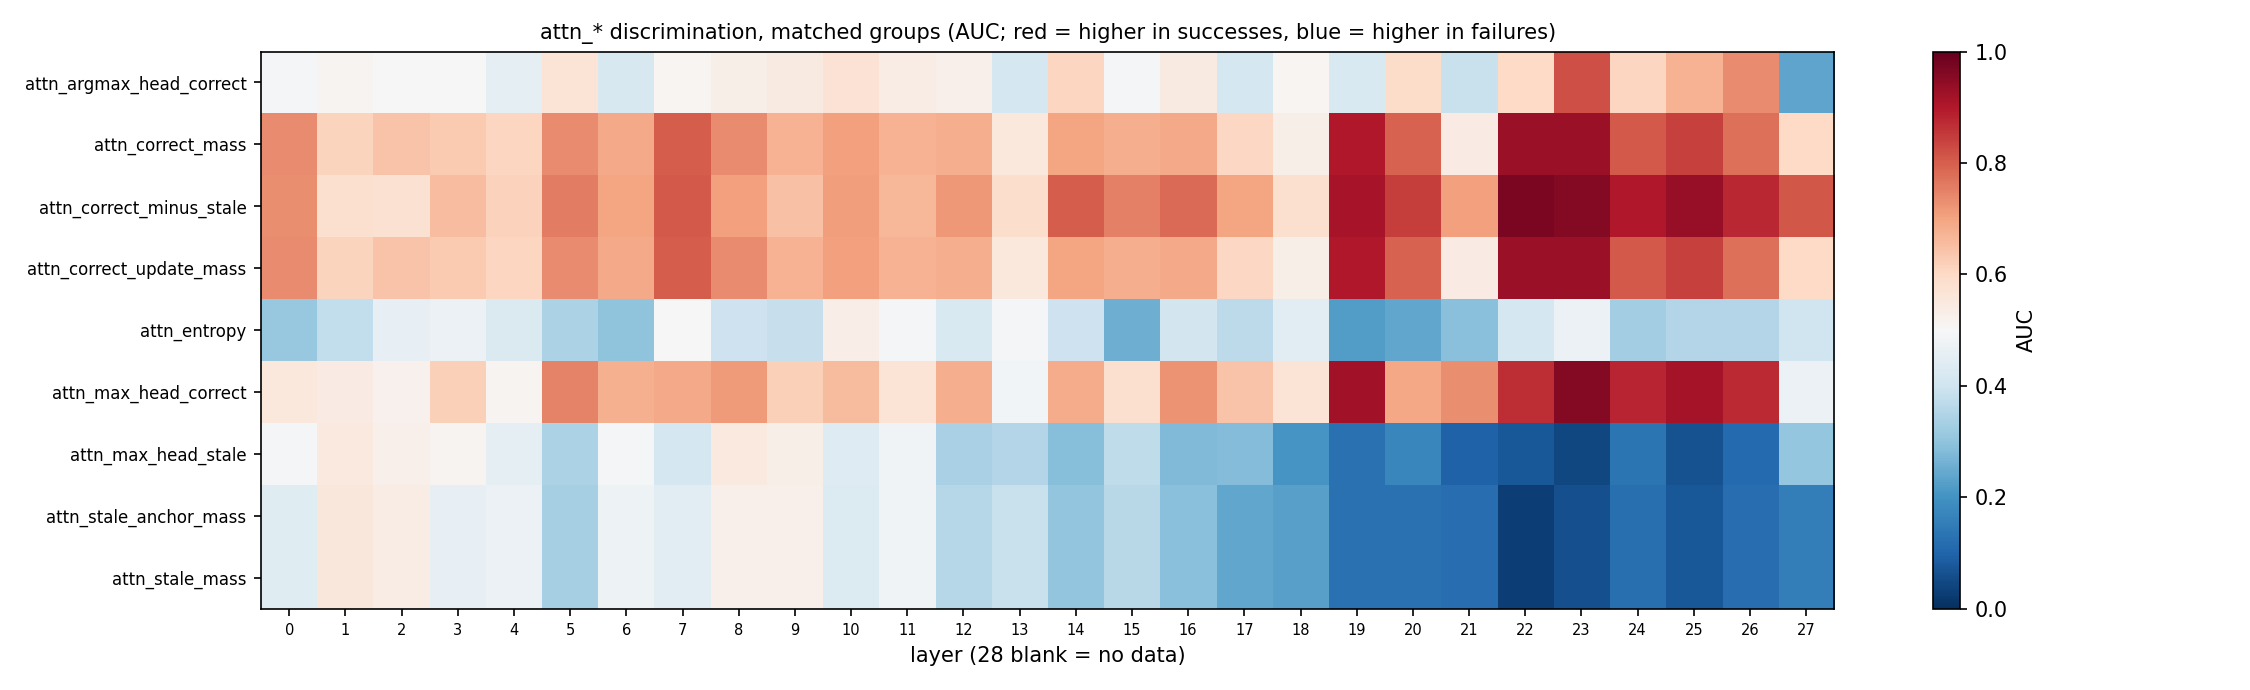
\includegraphics[width=\textwidth]{../reports/attn_sweep_matched.png}
\caption{Full matched attention sweep. Discrimination is concentrated at layers 19--25 and
is close to chance through the early and middle stack.}
\end{figure}

\section{What Survives}
\label{sec:survive}

\begin{table}[h]
\centering\small
\begin{tabular}{lrrrrl}
\toprule
Measure & Layer & Raw & Matched & Held-out & Verdict \\
\midrule
\code{attn\_correct\_minus\_stale} & 22 & $0.994$ & $0.973$ & $0.970$ & \pass{survives all three controls} \\
\code{jlens\_margin}              & 5  & $0.958$ & $0.888$ & $0.882$ & \pass{survives all three controls} \\
\code{logitlens\_margin}          & 18 & $0.690$ & $0.703$ & $0.669$ & \fail{fails split-half stability} \\
\bottomrule
\end{tabular}
\end{table}

Two defensible claims remain, and neither is the original one:

\begin{enumerate}[leftmargin=*,itemsep=2pt]
\item \textbf{Attention at layer 22 separates failures from successes} (matched AUC $0.973$,
      held-out $0.970$, layer stable in $90\%$ of splits). Failures place more attention mass
      on the stale anchor and less on the update mention. This is the strongest surviving
      result and it corroborates, on a properly matched and selection-corrected basis, the
      late-mid attention hypothesis previously advanced on weaker evidence.
\item \textbf{J-lens margin at layer 5 is predictive} (matched AUC $0.888$, held-out
      $0.882$, layer stable in $96\%$ of splits, replicating at $0.883$ with $682$ matched
      successes in the 5k run).
\end{enumerate}

\section{Limitations}
\label{sec:limits}

\paragraph{What J-lens measures.} By construction $\mathrm{jlens}_i = f_i(0) + J h_i$, where
$f_i$ executes decoder layers $i \ldots 28$ with the real KV cache. J-lens at layer 5
therefore includes the entire downstream network. We tested whether this makes it a
disguised readout of the output: it does not. The layer-specific component alone (after
removing each example's cross-layer mean) still yields AUC $0.911$, and cross-layer rank
correlation is \emph{lower} for J-lens ($0.425$) than for logit lens ($0.578$). The signal
is genuinely layer-local. Nonetheless the licensed statement is ``\emph{decodable through
the remaining network},'' not ``\emph{represented at layer 5}.'' Under the logit lens, which
does not route through downstream layers, matched internal AUC is $0.57$--$0.62$ everywhere
--- no usable internal signal.

\paragraph{Statistical power.} The matched 29-layer comparison rests on $72$ successes.
The 5k run supplies $682$ matched successes but only at layers 5, 8, and 13. The failure
population is capped at $137$: that is every failure the configuration produces, so a larger
failure sample requires a harder task setting, not merely more sampling.

\paragraph{Causality.} Everything reported here is correlational. A measure that predicts
the outcome need not participate in producing it. Moving from ``decodable'' to ``represented
and used'' requires activation patching or ablation, which requires GPU execution and is out
of scope for a CSV-only analysis.

\paragraph{Single model and dataset.} One model, one synthetic dataset, one prompt template.
The concentration of all failures in a single condition cell limits external validity
independently of the statistical issues.

\section{Recommendations}

\begin{enumerate}[leftmargin=*,itemsep=2pt]
\item \textbf{Retire the $137/137$ framing and the $2.3$ figure.} The first is untestable
      under its own null; the second is an artifact of including output-committed layers,
      where the correct state is the runner-up to an already-committed stale state.
\item \textbf{Report the layer-set with every rank statistic.} The $47{,}343$/$2.3$
      discrepancy was purely a sweep-depth difference and is otherwise unrecoverable from
      the numbers alone.
\item \textbf{Match on condition for every failure-vs-success comparison}, and report raw
      alongside matched so the confound size stays visible.
\item \textbf{Exclude layers 24--28 from any ``internal representation'' claim.} At layer 28
      the lens is the model's decision and every such statistic is circular.
\item \textbf{Target causal work at layer 22 attention}, the strongest and most stable
      surviving signal.
\end{enumerate}

\appendix
\section{Reproduction}

All results are reproducible from committed CSVs with no GPU. From the repository root:

\begin{quote}\code{python3 controls\_check.py \ \ \# round 1}\\
\code{python3 controls\_check2.py \ \# round 2 (matched)}\end{quote}

\code{controls\_check.py} implements the four controls of Section~\ref{sec:round1} and
recovers the true \code{dataset\_index} mapping. \code{controls\_check2.py} implements the
matched analysis, both permutation nulls (5{,}000 permutations), split-half selection
(500 splits), and the attention sweep, and writes a summary at
\code{reports/slack\_summary.txt}. Random seeds are fixed. Generated artifacts:
\code{controls\_output.txt}, \code{controls2\_output.txt}, \code{auc\_raw\_vs\_matched.csv},
\code{auc\_5k\_matched.csv}, \code{attn\_sweep\_matched.csv},
\code{failures\_fullsweep\_with\_true\_index.csv}, and the figures reproduced above.

\end{document}
